\documentclass[thesis.tex]{subfiles}
\begin{document}

\chapter{Pedestrian detection}
\label{sec:od}
In this chapter we describe the object detection problem and how we apply the discriptor to solve it.
Some introduction to object detection

Sliding window: $\sigma \cdot 134x70$ (128x64 + 3 pixel border)

\section{Support vector machine}

$L_2$-regularized $L_2$ loss support vector classifier from LIBLINEAR v. 1.94 \cite{fan2008liblinear}


\section{Performance measures}

\section{Dataset}
\label{sec:odDataset}

The dataset we use for training and testing our descriptor on the pedestrian detection application is called the \emph{INRIA Person Dataset}\footnote{\url{http://pascal.inrialpes.fr/data/human/}} (from now on called the INRIA dataset) constructed by \citet{dalal2005histograms}.
It concists of various real world images grouped into two subsets: Images with pedestrians (positives) and images without pedestrians (negatives). The positive images are rescaled cutouts centered around each pedestrian in larger images. The cutouts are first extracted and then individually re-scaled to make the pedestrian of each cutout 96 pixels in height from their feet to shoulders. The size of the cutouts are $64 \times 128$ pixels. In case a pedestrian cutout is smaller than the defined size after resizing, the borders are replicated to achieve the desired dimensions.
The positive set only contains images of somewhat upright persons that initially were at least 100 pixels in height. In order to improve the robustness of the dataset against reflected images, each positive cutout has its horizontally flipped image included as well.
The training dataset has a total of 2416 positives and 1218 negative images.
The test dataset has a total of 1126 positives and 453 negative images.


\Cref{fig:inriaExampleImages} shows examples of positive \subref{fig:inriaPositives} and negative \subref{fig:inriaNegatives} images from the INRIA dataset. From the positive examples we clearly see the high variety of upright positions and surroundings in the dataset.

\begin{figure}
	\centering
	\begin{subfigure}[t]{\textwidth}
		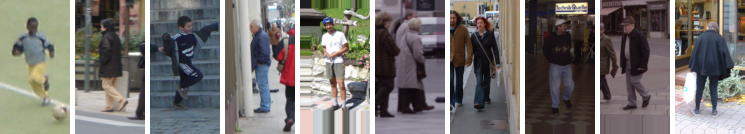
\includegraphics[width=\textwidth]{img/inriaPositives.png}
		\caption{Positives}
		\label{fig:inriaPositives}
		\vspace{2mm}
	\end{subfigure}
	\begin{subfigure}[t]{\textwidth}
		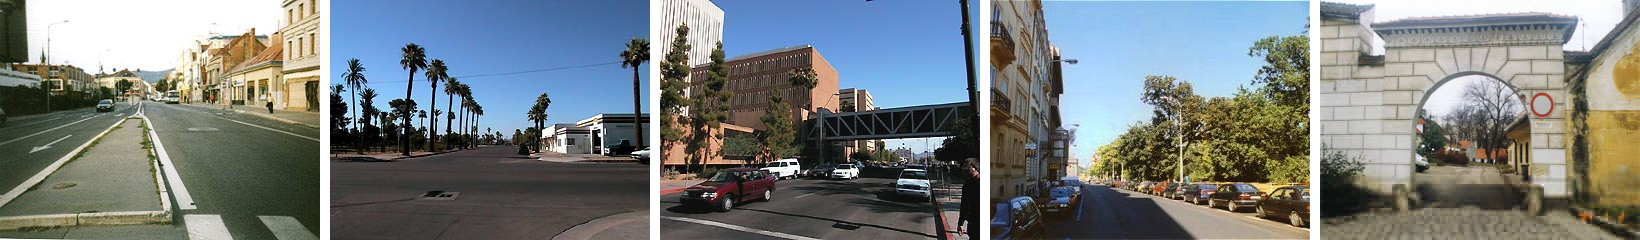
\includegraphics[width=\textwidth]{img/inriaNegatives.png}
		\caption{Negatives}
		\label{fig:inriaNegatives}
	\end{subfigure}
	\caption{Example INRIA images.}
	\label{fig:inriaExampleImages}
\end{figure}

\subsection{Pitfalls and deficiencies}
We have found two smaller problems with the INRIA dataset which could affect the results of using the dataset. The first problem is duplicate images. Amongst the negative training images we have found 10 pair-wise duplicates. This chould bias the svm since it effectively means that these images are weighted twice as high as the others. Given the small percentage of duplicates in the dataset the effect should however be close to nothing. In the initial training there are furthermore extracted windows at different random positions of the duplicates which decreases the bias even more. We have likewise found one duplicated image in the negative test set.

The second problem is the presence of people in some of the negatives.
\Cref{fig:inriaNegativePersons} show two examples of persons in the negative images of the INRIA dataset. The people are however either too small to fit correctly into the sliding window at any of the used scales or partially occluded by the image bounds to such an extend that we shouldn't be able to detect them anyway.

\begin{figure}[tb]
	\begin{subfigure}[t]{0.5\textwidth}
		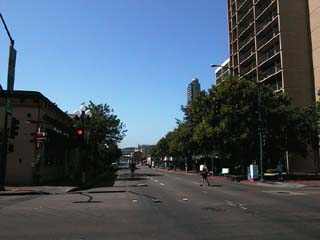
\includegraphics[width=\textwidth]{img/inriaManExample1.png}
	\end{subfigure}
	\begin{subfigure}[t]{0.5\textwidth}
		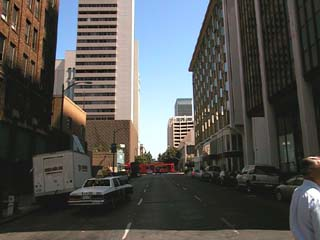
\includegraphics[width=\textwidth]{img/inriaManOccluded.png}
	\end{subfigure}
	\caption{Examples of persons in negative images}
	\label{fig:inriaNegativePersons}
\end{figure}

\section{Test setup}
Notes:

We follow \citet{dalal2005histograms}

Initial training: X randomly chosen windows per negative image and all positives
Hard training: Predict on sliding window of negatives ~ 2.2 million windows. Add hard negatives to training set and re-train.

Sliding window: 10 pixel in between windows. Multiscale.

Test on test set with sliding window on negatives ~ 1 million windows.

\section{Example}

\begin{figure}
	\centering
	\begin{subfigure}[t]{\textwidth}
		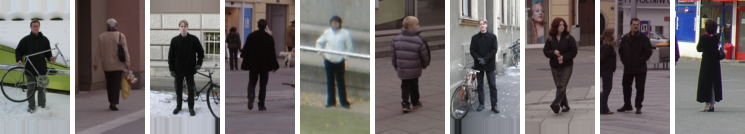
\includegraphics[width=\textwidth]{img/objectDetectionTP.png}
		\caption{True positives}
		\label{fig:objectDetectionTP}
		\vspace{2mm}
	\end{subfigure}
	\begin{subfigure}[t]{\textwidth}
		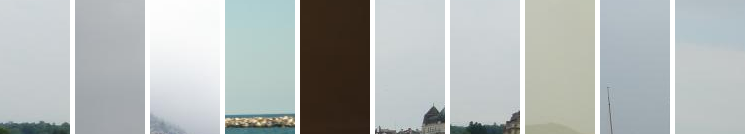
\includegraphics[width=\textwidth]{img/objectDetectionTN.png}
		\caption{True negatives}
		\label{fig:objectDetectionTN}
		\vspace{2mm}
	\end{subfigure}
	\begin{subfigure}[t]{\textwidth}
		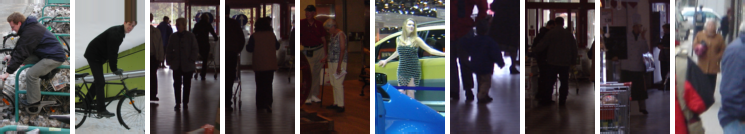
\includegraphics[width=\textwidth]{img/objectDetectionFN.png}
		\caption{False negatives}
		\label{fig:objectDetectionFN}
		\vspace{2mm}
	\end{subfigure}
	\begin{subfigure}[t]{\textwidth}
		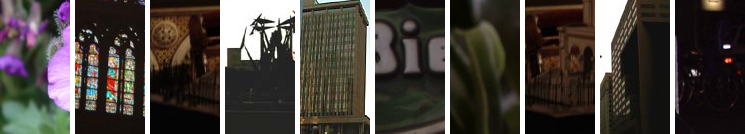
\includegraphics[width=\textwidth]{img/objectDetectionFP.png}
		\caption{False positives}
		\label{fig:objectDetectionFP}
	\end{subfigure}
	\caption{Example classifications of INRIA windows.}
	\label{fig:imageCorrespondenceCurves}
\end{figure}

\section{Parameter study}
\label{sec:odParameterStudy}

\subbibliography

\end{document}
